\section{Foundations of Bayesian Statistics}

\begin{definition}[Bayesian Network ~\cite{stephenson}]
A \textbf{Bayesian network} is a pair $B = (G,P)$ where $G=(V,E)$ is a DAG and $P$ is a joint probability distribution defined on a set of random variables $\mathcal{X}$. That is, it is a DAG and an associated joint probability distribution. \newline
\null \quad \quad Vertices in $G$ have a one-to-one correspondence to the random variables in $\mathcal{X}$ associated with $P$, meaning the set of vertices V represents both the vertices of $G$ and the random variables of the joint probability distribution $P$. \newline
\null \quad \quad $P$ factorizes on the sets $\{X \cup \prod\nolimits_{X}^{G}|X\in G\}$. That is, for each $X \in G$ there is a factor in $P$ that depends on $X$ and $\prod\nolimits_{X}^{G}$, namely $P_{X}(X|\prod\nolimits_{X}^{G})$.
\end{definition}

\begin{example}[Simple Bayesian Network] The DAG in Figure ~\ref{fig:bayesiannet1} paired with the joint probability distribution $p(X_{1}=x_{1},X_{2}=x_{2}) = p(X_{1}=x_{1})\cdot p(X_{2}=x_{2}|X_{1}=x_{1})$ is a Bayesian network. 

\begin{figure}[h!]
\centering
\begin{tikzpicture}
\Vertex[size=.5, color=white, label=$X$]{x1}
\Vertex[x = 2, size=.5, color=white, label=$Y$]{x2}
\Edge[Direct, distance=0.5](x1)(x2)
\end{tikzpicture}
\caption{}
\label{fig:bayesiannet1}
\end{figure}
\end{example}

\begin{remark}
In the context of this thesis, we only consider graphs $G$ which are finite DAGs (meaning $|V| < \infty)$ unless explicitly stated otherwise. Further, for our purposes, all such DAGs are directed graphical models with associated probability distributions. Therefore we will refer to DAGs $G=(V,E)$ and Bayesian networks interchangeably, with necessary details clarified in context. 
\end{remark}

\begin{definition}[Sample space, event~\cite{snell}]
Given a random experiment (an experiment whose outcome depends on chance), the \textbf{sample space} of the experiment is the set of all possible outcomes. Each subset of a sample space is called an \textbf{event}, that is, an outcome or a collection of outcomes of the random experiment. Therefore, event $\subseteq$ sample space. 
\end{definition}



\begin{example}
 In the context of Bayesian networks, we are interested in possible values of random variables which are represented by vertices. As a simple example, suppose we have the random binary variables $X$ and $Y$. Then the sample space of $X$ is $\{0,1\}$, and likewise for $Y$.  Generally, we will be interested in answering questions such as the probability that the random variable $X$ takes on a value $x \in \{0,1\}$; these queries are written $p(X=0)$, $p(X=1)$, or more generally, $p(X=x)$. Some possible queries one might encounter include the following:
\begin{itemize}
\item $p(X=x,Y=y)$, the probability that $X=x$ and $Y=y$ simultaneously, computed $p(X=x)\cdot p(Y=y)$,
\item $p(X=x|Y=y)$, the probability that $X=x$ given that we have observed the condition $Y=y$.
\end{itemize}

Let the marginal probabilities of these random vectors be given as follows:
\begin{align*}
&p(X=1) = \frac{3}{10} 	& p(X=0) = \frac{7}{10} \\
&p(Y = 0) = \frac{6}{10} 	&p(Y=1) = \frac{4}{10}
\end{align*}


\begin{table}[h!]
  \begin{center}
    \begin{tabular}{  c | c c c c}
	$X$ 		& 1 & 1 & 0 & 0 \\
	$Y$		& 1 & 0 & 1 & 0 \\
	\hline \\[-1em]
	$p(X,Y)$	&$ \frac{3}{25}$ & $\frac{21}{100}$ & $\frac{7}{25}$ & $\frac{21}{50}$
    \end{tabular}
  \end{center}
  \caption{The joint probability function $p(X,Y)$.}
  \label{jprobtable}
  \end{table}

where for $X$ and $Y$ binary variables, $p(X=1) = 1-p(X=0)$ since $\sum_{x\in\{0,1\}}p(X=x) = 1$. This joint probability function $p:\{0,1\} \times \{0,1\} \rightarrow [0,1]$ can also be encoded as a table, as in Table \ref{jprobtable}.\newline
\null \quad \quad This means that the joint probability function $p(X,Y)$ is not a value, but a function of the likelihood of potential values from the sample space of $Z$ and $Y$. Then, we can answer the query $p(X=1,Y=0)$ by reading off the table: $\frac{3}{25}$. \newline
\null \quad \quad Next, suppose we have observed the condition $Y=0$. Then, we can \textit{condition} the distribution, meaning we update the probability function such that it reflects our observation. We do so by looking at the scenarios in which $Y=0$:
\begin{align*}
	&p(X=0|Y=0) = \frac{21}{50}	& \text{and} &p(X=1|Y=0) = \frac{21}{100}.
\end{align*}
Then, using the fact that the probabilities should sum up to $1$,  we normalize:
\begin{align*}
p(X=0|Y=0) & \ \ = \ \ \frac{p(X=0|Y=0)}{p(X=0,Y=0) + p(X=1,Y=0)} \\[2em]
& \ \ = \ \ \frac{p(X=1,Y=0)}{p(Y=0)},
\end{align*}
and
\begin{align*}
p(X=1|Y=0) & \ \ = \ \ \frac{p(X=1,Y=0)}{p(X=0,Y=0) + p(X=1,Y=0)} \\[2em]
& \ \ = \ \ \frac{p(X=1,Y=0)}{p(Y=0)}.
\end{align*}
Thus, with $p(Y=0) = \frac{63}{100}$, these give us

\begin{table}[h!]
  \begin{center}
    \begin{tabular}{  c | c c c c }
	$X|Y=0$ 		& 1 & 0  \\
		\hline \\[-1em]
	$p(X|Y=0)$		& $\frac{2}{3}$  & $\frac{1}{3}$  \\
    \end{tabular}
  \end{center}
  \end{table}
\end{example}

\begin{definition}[(Probabilistic) query]
A probabilistic query $q$ on a graph $G=(V,E)$ is an inference question of the form $p(X_{1}, ..., X_{m}|Y_{1}, ..., Y_{n})$ where $X_{i}, i \in [0,m] \in V$ and $Y_{j}, j \in [0,n] \in V.$ $X_{i}$ are the \textbf{targets} of $q$ while $Y_{j}$ are the \textbf{conditions} or \textbf{observations}. 
\end{definition}

\begin{theorem}[Bayes' Theorem~\cite{snell}] Given two random variables $X$ and $Y$ with $p(Y) \neq 0$
$$p(X|Y) = \frac{p(Y|X) \cdot p(X)}{p(Y)}.$$
\end{theorem}

\begin{remark}
Bayes' Theorem will serve as a significant basis for many of the calculations necessary for transforming graphs in later chapters. 
\end{remark}

\begin{definition}[(Statistical) independence~\cite{snell}]\label{statisticalindependence}
Let $X$ and $Y$ be random variables. Then $X$ and $Y$ are called \textbf{independent} whenever 
$$P(X,Y) = p(X)p(Y)$$ 
or equivalently if
$$ p(X) = p(X|Y)$$
and vice versa.
\end{definition}

\begin{remark}
~\ref{statisticalindependence} can be intuitively understood as follows: learning about $Y$ has no effect on our knowledge concerning $X$ and vice versa.
\end{remark}

\begin{definition}[Conditional independence~\cite{snell}]\label{conditionalindependence} 
Let $X$, $Y$, and $Z$ be random variables. Then $X$ is said to be \textbf{conditionally independent} of $Y$ given $Z$ iff $p(X|Y,Z) =p(X|Z)$.
Otherwise, they are said to be \textbf{conditionally dependent}. 
\end{definition}

\begin{remark}
Definition~\ref{conditionalindependence} can be intuitively understood as follows: if we know about $Z$, then learning about $Y$ has no effect on our expectation concerning $X$. Likewise, learning about $X$ has no effect on our expectation concerning $Y$ if we know about $Z$. 
\end{remark} 

\begin{remark} Definition ~\ref{statisticalindependence} and Definition ~\ref{conditionalindependence} also hold for disjoint sets $A,B$, and $C \subset V$ with $p$ a joint probability distribution defined on $V$. 
\end{remark}

\begin{example} Suppose Evin and Lisa take turns flipping a single coin which either results in heads ($H$) or tails ($T$). Naturally, one would assume that the probability of Lisa flipping heads is independent of the probability that Evin flips heads, that is, $$p(Lisa = H|Evin = H) = p(Lisa = H),$$ since flipping a fair coin once does not dictate the outcome of a second flip. This means the two experiments are independent.\newline
\null \quad \quad Now suppose we learn that the the coin is biased, calling the presence of the bias event $Z$. If the first coin flip results in heads, we would guess that the coin is more likely biased toward heads, and expect that the second coin flip to be heads. That is, the event of Evin flipping heads gives us information about the likelihood that Lisa will flip heads, given that we have observed $Z$. Then, whereas $p(Evin=H)$ and $p(Lisa=H)$ were previously independent from one another, observing event $Z$ makes them depend on one another. Therefore the two events are conditionally dependent given $Z$:
$$p(Lisa=H|Z,Evin=H) \neq p(Lisa=H|Evin=H).$$ 

\begin{center}
\begin{figure}[h!]
\begin{center}
\centering
\includegraphics[width=0.8\textwidth]{cointoss.jpeg}
\caption{Evin and Lisa engaging in a game of chance.}
\end{center}
\end{figure}
\end{center}

\end{example} 
\null \quad \quad Dependence, independence, and conditional independence have an intuitive manifestation within graph structure, which follows from Definition ~\ref{statisticalindependence}: \newline
\null \quad \quad Given a graph $G=(V,E)$ such as any of the graphs in Figure~\ref{fig:ind}, if two vertices $X, Y \in V$ have an edge between them, either $(X,Y)$ or $(Y,X)$, then they are dependent variables by construction of our graphs. \newline
\null \quad \quad If there exists a route between two vertices $X$ and $Y$, but $X$ and $Y$ are not adjacent, then they are conditionally independent, where the conditions are the vertices on that route. This is because information about $X$ can give us information about an intermediary node on the route and allow us to gain information about $Y$ (or vice versa). \newline
\null \quad \quad Finally, if two vertices are not connected by a route (disconnected) then they are independent, since information about $X$ cannot give us information about $Y$ under any circumstances. \\[2em]

\begin{figure}[h!]
\centering

\begin{center}
\begin{tikzpicture}
\Vertex[x=-4.5, y=-.7, size=.5, color=white, label=$X$]{x1}
\Vertex[x = -2.5, y=-.7, size=.5, color=white, label=$Y$]{x2}
\Edge[Direct, distance=0.5](x1)(x2)

\Vertex[size=.5, color=white, label=$X$]{x1}
\Vertex[x = 2, size=.5, color=white, label=$Y$]{x2}
\Vertex[y = -1.5, x=1 ,size=.5,color=white]{x3}
\Edge[Direct, distance=0.5](x1)(x3)
\Edge[Direct, distance=0.5](x3)(x2)

\Vertex[x = 3,size=.5, color=white, label=$X$]{x1}
\Vertex[x = 5, size=.5, color=white, label=$Y$]{x2}
\Vertex[y = -1.5, x=3, size=.5,color=white]{x3}
\Vertex[y = -1.5, x=5, size=.5,color=white]{x4}
\Edge[Direct, distance=0.5](x1)(x3)
\Edge[Direct, distance=0.5](x3)(x4)
\Edge[Direct, distance=0.5](x2)(x4)

\Vertex[x = 7.3, y=-.7, size=.5, color=white, label=$X$]{x1}
\Vertex[x = 8.7, y =-.7, size=.5, color=white, label=$Y$]{x2}


\Text[x=-3.5 ,y=-3]{dependent}

\Text[x=2.5 ,y=-3]{$X$ and $Y$ conditionally independent}

\Text[x=8 ,y=-3]{independent}

\end{tikzpicture}
\end{center}

\caption{}
\label{fig:ind}
\end{figure}


